\documentclass[]{article}
\usepackage[UTF8]{ctex}
\usepackage{amsmath}

\usepackage{amsmath}
\usepackage{graphicx}
\newtheorem{theorem}{Theorem}
\renewcommand{\thesection}{\Roman{section}}

%opening
\title{密码学新方向}
\author{WHITFIELD DIFFIE AND MARTIN E. HELLMAN, \\
{\small  翻译:李晓峰(cy\_lxf@163.com)}\\
{\small 译者单位:北京联合大学智慧城市学院}\footnote{译文来自于经典文献翻译项目https://gitee.com/uisu/InfSecClaT,欢迎大家加入经典翻译项目,为更多的人能够获取这些经典文献所传递信息做一点贡献。}
}

\usepackage{hyperref} %生产书签

\begin{document}
	
	\maketitle
	
	\begin{abstract}
		本文讨论了密码学现代发展的两个方面。远程处理的广泛应用促使开发新型密码系统,这些系统最大限度地减少了对安全密钥分发通道的需求,提供了等同于书面签名的功能。本文提出了解决这些当前未解决问题的方法。同时,本文也讨论了通信和计算理论开始提供解决长期存在的密码学问题的工具。
	\end{abstract}

	\section{引言}
	我们今天站在密码学革命的边缘。廉价数字设备的发展使其摆脱了机械计算的设计限制,并将高级密码设备的成本降至可用于远程提款机和计算机终端等商业应用。相应地,这些应用程序为新型密码系统的需求创造了条件,这种系统最大程度地减少了安全密钥分发通道的必要性,并提供了等同于书面签名的功能。与此同时,信息理论和计算机科学的理论进展表明,可能提供可证明安全的加密系统,这将把这门古老的艺术变成一门科学。
	
	计算机控制的通信网络的发展为世界两端的人或计算机之间提供了轻松、廉价的联系方式,取代了大部分的邮件和许多短途通信旅行活动(many excursions with telecommunications)。对于许多应用而言,这些联系必须安全可靠,不能被窃听和注入非法信息。然而,目前安全问题的解决在通信技术的其他领域中依然相对滞后。当代的密码学无法满足要求,因为其使用会给系统用户带来如此严重的不便,以至于会消除远程处理的许多好处。
	
	最著名的密码问题是隐私问题:防止未经授权从不安全信道上的通信中提取信息。然而,为了使用密码学来确保隐私,目前通信各方必须共享一个其他人不知道的密钥。这是通过一些安全通道(如私人快递或挂号信)提前发送密钥来完成的。私人谈话然,在商业中,两个素不相识的人之间是很常见的,这是不现实的。期望最初的业务联系被推迟足够长的时间,以便通过某种物理手段传输密钥。这种密钥分配问题所带来的成本和延迟是将商业通信转移到大型远程处理网络的主要障碍。
	
	第三节提出了两种在公共(即不安全)信道上传输密钥信息而不损害系统安全性的方法。在公钥密码系统中,加密和解密由不同的密钥E和D控制,使得从E计算D在计算上是不可行的(例如,需要$10^{100}$条指令)。因此,加密密钥E可以在不泄露解密密钥D的情况下公开。因此,网络的每个用户可以将其加密密钥放在公共目录中。这使得系统的任何用户能够以只有预期的接收者才能破译的方式向任何其他用户发送消息。因此,公钥密码系统是多路访问密码。因此,任何两个人之间都可以进行私人谈话,无论他们以前是否交流过。每一方向另一方发送消息,用接收方的公开加密密钥加密,并用自己的秘密解密密钥解密自己收到的消息。
	
	我们提出了一些开发公钥密码系统的技术,但这个问题在很大程度上仍然是公开的。
	
	公钥分发系统提供了一种不同的方法来消除对安全密钥分发信道的需要。在这样的系统中,希望交换密钥的两个用户来回通信,直到他们得到共同的密钥。窃听该交换的第三方必须发现从偷听到的信息计算密钥在计算上是不可行的。第三节给出了公钥分配问题的一种可能的解决方案,Merkle[1]给出了不同形式的部分解。
	
	第二个问题是身份验证,该问题可以通过密码解决,它阻碍了远程处理系统取代当代商业通信。在目前的商业中,合同的有效性是通过签字来保证的。签署的合同作为协议的法律证据,持有人可在必要时在法庭上出示。然而,使用签名需要传输和存储书面合同。为了有一个纯粹的数字替代这种纸质仪器,每个用户必须能够产生一个信息,其真实性可以由任何人检查。由于只有一个人可以发出消息,但许多人可以接收消息,因此这可以被视为广播密码。目前的电子认证技术不能满足这一需要。
	
	第四节讨论了提供真实的、数字的、依赖电文的签名的问题。由于这里提出的原因,我们将其称为单向身份验证问题。给出了一些部分解决方案,并说明了如何将任何公钥密码系统转换为单向认证系统。
	
	第五节将考虑各种密码问题的相互关系,并介绍更困难的陷门问题。
	
	在通信和计算产生了新的密码学问题的同时,它们的衍生(their offspring),信息论和计算理论已经开始为解决经典密码学中的重要问题提供工具。
	
	寻找无法破解的密码是密码学研究中最古老的主题之一,但直到本世纪,所有提出的系统最终都被破解了。然而,在二十世纪二十年代,“一次一密”(ont time pad)被提出来,并被证明是牢不可破的[2,pp。398-400].四分之一世纪后,信息论[3]为这一系统和相关系统的理论基础奠定了坚实的基础。“一次一密”需要极长的密钥,因此在大多数应用中都非常昂贵。
	
	相反,大多数密码系统的安全性在于密码分析者在不知道密钥的情况下发现明文是计算困难的。这个问题属于计算复杂性和算法分析领域,这两个最近的学科研究解决计算问题的难度。使用这些理论的结果,在可预见的未来,有可能将安全性的证明扩展到更有用的系统类别。第六节探讨了这种可能性。
	
	在论文继续阐述之前,我们先在下一节中介绍术语并定义威胁环境。
	
	
	\section{传统密码体系}
	
	密码学是对“数学”系统的研究,用于解决两种安全问题:隐私和认证。保密系统防止未经授权的各方从通过公共信道传输的消息中提取信息,从而向消息的发送者保证该消息仅由预期的接收者读取。认证系统可防止未经授权将消息注入公共信道,从而向消息的接收者保证其发送者的合法性。
	
	
	如果信道的安全性不足以满足用户的需求,则该信道被视为公共信道。因此,诸如电话线之类的信道可能被一些用户认为是私有的,而被其他用户认为是公共的。任何信道都可能受到窃听或注入的威胁,或者两者兼而有之,具体取决于其使用情况。在电话通信中,注入的威胁是最重要的,因为被叫方无法确定正在呼叫哪个电话。窃听需要使用窃听器,在技术上更困难,在法律上也更危险。相比之下,在无线电领域,情况正好相反。窃听是被动的,不涉及法律风险,而注入会使非法发射器被发现和起诉。
	
	
	将我们的问题分为隐私和认证,我们有时会进一步将认证细分为消息认证和用户认证,上面说的认证问题是消息认证,对于用户认证,系统的唯一任务是验证个人是否是他所声称的。例如,必须验证出示信用卡的个人的身份,但没有他希望发送的消息。尽管用户身份验证中明显没有消息,但这两个问题在很大程度上是等价的。在用户认证中,有一个隐含的消息“我是用户X”,而消息认证只是验证消息发送方的身份。然而,这两个子问题在威胁环境和其他方面的差异有时使区分它们变得容易。
	
	图\ref{Fig:fig1}说明了传统密码系统用于保密通信时的信息流动情况。有三方:发射机、接收机和窃听器。发送器生成要通过不安全信道传送到合法接收器的明文或未加密消息P。为了防止窃听者获知P,发射机对P进行可逆变换$S_K$,以产生密文(ciphertext)或密码(cryptgram)$C=S_K(P)$。密钥K通过安全通道在线传输到合法接收器,如图1中屏蔽路径所示。由于合法接收者知道K,他可以通过$S_K^{-1}$操作来解密C,以获得原始明文消息$S_K^{-1}(C)=S_K^{-1}(S_K(P))=P$。由于容量或延迟的原因,安全信道不能用于传输P本身。例如,安全通道可能是每周快递,而不安全通道则是电话线。
	
	\begin{figure}[htbp]
		\centering
		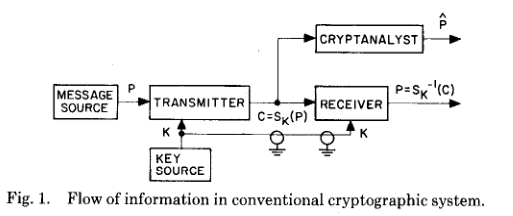
\includegraphics[width=0.8\textwidth]{FIG1.png}
		\caption{传统加密系统中的信息流}
		\label{Fig:fig1}
	\end{figure}
	
	一个密码系统是一个有可逆变换的单参数族
	\begin{equation}
		S_K:{P}\rightarrow {C}
	\end{equation}
	是从消息明文空间$\{P\}$到密文空间$\{C\}$的一个变换。参数$K$被称为密钥(key),是从有限集合$\{K\}$中选择的,这个有限集合$\{K\}$称为密钥空间,如果$\{P\}$和$\{C\}$相等,我们将其记为$\{M\}$,当讨论某一个加密变换$S_K$时,我们有时将省略对系统的提及,而仅提及变换K。
	
	
	设计密码系统$\{S_K\}$的目标是使加密和解密操作成本低廉,但确保任何成功的密码分析操作都过于复杂而不经济。解决这个问题有两种方法。一种是由于密码分析的计算成本(过高)而安全,这种系统称为计算安全的(computationally secure),但会屈服于无限计算的攻击;而一个无论允许多少计算量都能抵抗任何密码分析攻击的系统被称为无条件安全的(unconditionally secure.)。在[3]和[4]中讨论了无条件安全系统,它属于信息论的一部分,称为香农理论,该理论涉及可通过无限计算获得的最优性能。
	
	无条件安全源于一个密文存在多个有意义的解。例如,由英语文本产生的简单替换密码XMD可以表示明文消息:NOW、AND、THE等。相反,计算安全的密文包含足够的信息来唯一地确定明文和密钥,它的安全性完全取决于计算它们的成本。
	
	
	通常使用的唯一无条件安全系统是“一次一密”,其中明文与随机选择的相同长度的密钥相结合。虽然这样的系统可证明是安全的,但所需的大量密钥使其对于大多数应用来说是不切实际的。除非另有说明,本文讨论计算安全系统,因为这些系统更普遍适用。当我们谈到需要开发可证明安全的密码系统时,我们排除了那些难以使用的密码系统,例如“一次一密”。相反,我们认为系统只使用几百位密钥,并且可以在少量数字电路或几百行软件中实现。
	
	如果通过使用的内存量或运行时间来衡量的成本是有限的,但大得不可思议,则我们称该任务在计算上是不可行的(computationally infeasible )。
	
	就像纠错码分为卷积码和分组码一样,密码系统也可以分为两大类:流密码和分组密码。流密码以小块(位或字符)的形式处理明文,通常产生位的伪随机序列,该序列以模2的形式添加到明文的比特位上。分组密码以纯组合的方式作用于大的文本块,以这样一种方式,输入块中的小变化产生结果输出中的大变化\footnote{译者注:这就是密码学中的通常所说的变换具有的雪崩效应,密码中的雪崩效应是指,当密码中的一位或几位发生变化时,导致整个密码的值都会发生显著变化。也就是说,小的密码变化会引发大的密码值变化。这种现象是密码学中的一种重要特性,因为它可以确保密码的安全性。如果密码中的某一位或几位被修改,即使只有一小部分的变化,也会导致整个密码的值发生了巨大的变化,从而使攻击者难以推断密码的原始值。S盒通常具有雪崩效应。S盒是在DES(数据加密标准)和AES(高级加密标准)这样的对称加密算法中使用的一个重要的密码学组件。S盒的作用是把一些输入位映射到一些不同的输出位,从而增强加密算法的安全性。在S盒的设计中,通常需要确保任何一个输入位的变化都能够产生尽可能多的输出位的变化。这样,当输入发生变化时,输出也会发生明显的变化,从而产生雪崩效应。这一特性可以使攻击者难以通过修改输入密码的几位来得出原始密码的值,从而大大增强了密码体系的安全性。}。本文主要讨论分组密码,因为这种错误传播特性在许多认证应用中是有价值的。
	
	
	在认证系统中,使用密码学来保证消息的真实性。不仅必须防止干扰者将全新的、看似真实的消息注入到信道中,还必须防止他通过组合、复制过去的旧消息,仅仅重复已有的消息来制造看似真实的消息。一个旨在保障私密性的密码系统通常不会防止这种后一种的恶意行为。
	
	为了保证消息的真实性,需要添加信息,这些信息不仅是消息和密钥的函数,还包括日期和时间。例如,可以将日期和时间附加到每个消息并对整个序列进行加密。这可以确保只有拥有密钥的人才能生成解密后包含正确日期和时间的消息。然而,需要注意使用一个系统,在该系统中,密文中的小变化会导致明文大的变化。这种故意的误差扩散确保,如果有意注入通道上的噪声将一个消息如“删除文件 7”更改为另一个消息如“删除文件 8”,它也会破坏身份验证信息。消息将被拒绝认为是不真实的。
	
	评估密码系统的充分性的第一步是对其所面临的威胁进行分类。用于隐私或认证的加密系统可能会受到以下威胁。
	
	\textbf{仅密文攻击(ciphertext only attack )}是密码分析者仅拥有密文的密码分析攻击。
	
	\textbf{已知明文攻击(known plaintext attack )}是密码分析攻击,其中密码分析者拥有大量相应的明文和密文。
	
	\textbf{选择明文攻击(chosen plaintext attack )}是一种密码分析攻击,其中密码分析者可以提交他自己选择的无限数量的明文消息,并检查得到的密码。
	
	在所有情况下,假设对手知道所使用的一般系统$\{S_K\}$,因为该信息可以通过研究密码设备来获得。虽然密码学的许多用户试图对他们的设备保密,但许多商业应用不仅要求通用系统是公开的,而且要求它是标准的。
	
	仅密文攻击在实践中经常发生。密码分析员仅使用所使用的语言的统计特性的知识(例如,在英语中,字母E出现的频率为13\%)和某些“可能”单词的知识(例如,字母可能以“ Dear Sir:”开头)。它是系统所能承受的最弱的威胁,任何抵挡不住(succumbs)它的系统都被认为是完全不安全的。
	
	
	一个安全系统应能够抵御已知明文攻击,使其用户不必为保守过去的消息而感到负担,或在解密之前对这些消息进行复述。这对于系统的用户来说是一个不合理的负担,特别是在商业环境中,产品公告或新闻稿可能以加密形式发送,以供以后公开披露。类似的情况在外交信函中也已经出现,这导致了许多被认为是安全的系统遭到破解。虽然已知明文攻击并非总是可行的,但其发生频率足以使未能抵御此类攻击的系统被认为不安全。
	
	实践中很难实现选择明文攻击,但可以近似实现。例如,向竞争对手提交一个提案,可能会导致他将其加密后传输到总部。一个安全的密码系统应能够抵御选择明文攻击,以避免用户担心其对手在系统中执行消息注入攻击。
	
	为了证明系统是安全的,考虑更强大的密码分析威胁是适当的,因为这些不仅给出了密码系统工作环境的更真实的模型,而且使系统强度的评估更容易。许多系统使用仅密文攻击是困难的,但是在已知明文或者选择明文攻击下就立即被淘汰了。
	
	从这些定义中可以看出,密码分析是一个系统识别问题。已知明文攻击和选择明文攻击分别对应被动和主动系统识别问题。与许多其他被认为是系统识别的学科(例如自动故障诊断)不同,密码学的目标是构建难以识别的系统,而不是易于识别的系统。
	
	选择明文攻击通常被称为敌我识别攻击,这一术语起源于第二次世界大战后,密码“敌我识别”系统的发展。敌我识别系统使军用雷达能够自动区分友机和敌机。雷达向飞机发送时变询问,飞机接收该询问,在适当的密钥下对其进行加密,并将其发送回雷达。通过将该响应与正确加密的挑战版本进行比较,雷达可以识别友机。当飞机在敌方领土上空时,敌方密码分析员可以发送挑战并检查加密响应,以试图确定正在使用的认证密钥,从而对系统进行选择明文攻击。在实践中,这种威胁是通过限制挑战的形式来应对的,挑战不需要是不可预测的,而只需要是不重复的。
	
	
	认证系统还面临着传统密码学无法解决的其他威胁,这些威胁需要求助于本文介绍的新思想和新技术。在多用户网络中,接收方通常是系统本身,因此接收方的密码表(password tables)和其他认证数据比发送方(个人用户)的密码表和其他认证数据更容易被窃取。如后面所示,一些用于防止这种威胁的技术也可以防止争议的威胁(threat of dispute.),即,消息可以被发送,但随后被发送方或接收方否认。或者,任何一方都可能声称发送了一条消息,而事实上根本没有发送。需要不可伪造的数字签名和收据。例如,不诚实的股票经纪人可能试图通过伪造客户的订单来掩盖未经授权的买卖,以谋取私利,或者客户发现该订单会造成损失,从而否认他实际授权的订单。我们将介绍一些概念,这些概念允许接收者验证消息的真实性,但防止他生成认证消息,从而防止接收者的认证数据泄露威胁和争议威胁。
	
	\section{公钥密码体系}
	
	如图1所示,密码学已经成为一种衍生的安全措施。一旦存在可以传输密钥的安全信道,就可以通过加密,将安全性扩展到具有更高带宽或更小延迟的其他信道。其效果是将密码学的使用限制在事先为密码安全做好准备的人之间的通信中。
	
	为了发展大型、安全的电信系统,必须改变这一点。大量的用户$n$,导致更大数量,$(n^2-n)/2$,的签字密钥对,这些用户可能希望与所有其他人私下通信。假设先前不认识的一对用户将能够等待通过某种安全物理手段发送的密钥,或者可以预先安排所有$(n^2-n)/2$对的密钥,这是不现实的。在另一篇论文[5]中,作者考虑了一种保守的方法,该方法不需要密码学本身的新发展,但这会降低安全性,带来不便,并将网络限制为与初始连接协议相关的星形配置。
	
	我们提出,可以开发图2所示类型的系统,其中仅通过公共信道通信并且仅使用公开技术就可以创建两方安全连接。我们研究了解决这个问题的两种方法,分别称为公钥密码系统和公钥分发系统。第一个功能更强大,有助于解决下一节中讨论的认证问题,而第二个则更接近于实现。
	
	一个公钥密码系统(public key cryptosystem)是一对在有限消息空间$\{M\}$上的算法族,$\{E_K\}_{K\in \{K\}}$和$\{D_K\}_{K\in \{K\}}$,代表可逆变换,
	\begin{align}
		E_K : \{M\}\rightarrow \{M\}\\
		D_K :\{M\}\rightarrow \{M\}
	\end{align}
	并且满足:
	\begin{itemize}
		\item 对于每一个$K\in \{K\}$,$E_K$是$D_K$的逆;
		\item 对于每一个$K\in \{K\}$和$M\in \{M\}$,算法$E_K$和$D_K$是容易计算的;
		\item 对于几乎每一个$K\in \{K\}$,等效于$D_K$的每个容易计算的算法,从$E_K$推导出来这些算法在计算上不可行;
		\item 对于每一个$K\in \{K\}$,从$K$计算逆对$E_K$和$D_K$是可行的。
	\end{itemize}


	由于第三个特性,用户的加密密钥$E_K$可以公开而不损害其秘密解密密钥$D_K$的安全性。因此,密码系统被分成两个部分,一族加密变换和一族解密变换,这样,给定一族的成员,不可能找到另一族的相应成员。
	
	第四个性质保证,当加密或解密变换不受约束时,有一种可行的方法来计算相应的逆变换对。在实践中,加密设备必须包含一个真正的随机数生成器(例如,有噪声的二极管)来生成$K$,以及用于从其输出生成$E_K-D_K$对的算法。
	
	给定这样一个系统,密钥分配问题就大大简化了。每个用户在其终端生成一对逆变换,即E和D。解密变换D必须保密,但不需要通过任何渠道进行通信。加密密钥E可以通过将其与用户的姓名和地址一起放在公共目录中而被公开。然后,任何人都可以加密消息并将其发送给用户Bob,但没有其他人可以破译为Bob提供的消息\footnote{译者注:原文Anyone can then encrypt messages and send them to the user, but no one else can decipher messages intended for him.根据上下文意思“the user”和"him"是指同一人,为了便于准确翻译和理解,我们称其为Bob。}。因此,公钥密码系统可以被视多用户共享密码( multiple access ciphers.)。
	
	
	保护加密密钥的公共文件不受未经授权的修改是至关重要的。由于文件的公共性质,这项任务变得更加容易。读取保护是不必要的,而且由于文件很少被修改,因此可以经济地使用精心设计的写入保护机制。
	
	公钥密码系统的一个提示性的例子,尽管不幸的是没有用,是通过将明文乘以可逆的二进制$n\times n$矩阵E来加密明文,明文表示为二进制n维向量m。因此,密码等于$Em$。设$D=E^{-1}$,我们有$m=DC$。因此,加密和解密都需要大约$n^2$次操作。然而,从E计算D涉及矩阵求逆,这是一个更困难的问题。
	并且至少在概念上,获得任意一对逆矩阵比对给定矩阵求逆更简单。从单位矩阵I开始,进行初等行、列运算,得到任意可逆矩阵E。
	然后从I开始,以相反的顺序做这些相同的初等运算的逆运算,得到$D=E^{-1}$。基本操作的序列可以很容易地从随机位串中确定。
	
	
	不幸的是,矩阵求逆只需要$n^3$个运算。“密码分析”时间(即从E计算D)与加密或解密时间的比率最大为n,并且需要巨大的块大小才能获得$10^6$或更大的比率。
	此外,用于从I获得E的基本运算的知识似乎并不能大大减少计算D的时间。并且,由于在二进制算术中没有舍入误差,因此在矩阵求逆中数值稳定性并不重要。尽管缺乏实用性,这个矩阵例子对于阐明公钥密码系统中必要的关系仍然是有用的。
	
	一种更实用的方法是找到一对易于计算的逆算法E和D,使得从E中推导出D很困难,这利用了用低级语言分析程序的困难。任何试图确定别人的机器语言程序实现了什么操作的人,都知道E本身(即E所做的事情),但很难从E的算法中推导出来。如果通过添加不必要的变量和语句使程序有意混淆,那么确定逆算法可能会变得非常困难。当然,E必须足够复杂,才能防止从输入输出对中识别出它。
	
	从本质上讲,所需要的是一个单向编译程序:它把用高级语言编写的容易理解的程序翻译成用某种机器语言编写的难以理解的程序。编译器是单向的,因为它必须能够进行编译,但不能反向编译。由于在该应用中,程序大小和运行时间的效率不是至关重要的,因此如果机器语言的结构可以被优化以帮助混淆,则这样的编译器是可能的。
	
	Merkle [1]独立地研究了在不安全信道上分配密钥的问题。该方法不同于上面建议的公钥密码系统的方法,并且将被称为公钥分发系统(public key distribution system)。
	目标是让两个用户A和B通过不安全的信道安全地交换密钥。然后,该密钥由正常密码系统中的两个用户用于加密和解密。
	Merkle提出了一种解决方案,其密码分析成本增长为$n^2$,其中$n$是合法用户的成本。
	不幸的是,系统的合法用户的成本在传输时间上与在计算上一样多,因为Merkle的协议需要在决定一个密钥之前传输n个潜在密钥。
	Merkle指出,这种高传输开销妨碍了该系统在实践中非常有用。如果在建立协议的开销上设置1兆比特的限制,则该技术可以实现大约10000比1的成本比,这对于大多数应用来说太小了。如果廉价的高带宽数据链路变得可用,则可以实现百万分之一或更大的比率,并且该系统将具有相当大的实用价值。
	
	
	我们现在提出一种新的公钥分配系统,它具有几个优点。首先,它只需要交换一把“钥匙”。其次,在合法用户的努力中,密码分析的努力似乎呈指数增长。第三,它的使用可以绑定到用户信息的公共文件,该公共文件用于向用户B认证用户A,反之亦然。通过使公共文件本质上成为只读存储器,一次个人出现允许用户向许多用户多次认证其身份。Merkle的技术要求A和B通过其他手段验证对方的身份。
	
	
	新技术利用了在具有素数q个元素的有限域GF(q)上计算对数明显是困难的这一结论。设
	\begin{equation}
		Y=\alpha^X \pmod{q}\ \ ,for\ 1\leq X\leq q-1
	\end{equation}
	此处$\alpha$是GF(q)中固定的素元素,X是以$\alpha$为基Y的对数,模q:
	\begin{equation}
		X=log_\alpha Y \pmod{q}\ \ ,for\ 1\leq Y\leq q-1
	\end{equation}
	从X计算Y是容易的,进行$2\times log_2 q$次乘法运算[6,pp.398-422]。例如,X=18,
	\begin{equation}
		Y=\alpha ^{18}=(((\alpha^2)^2)^2)^2 \times \alpha^2
	\end{equation}
	另一方面,从Y计算X很困难,对于一些仔细选择的q,在使用最好的算法情况下[7,pp.9,575-576,[8]],需要$q^{1/2}$个顺序运算。
	
	我们技术的安全性关键取决于计算模q对数的困难程度,如果有一种算法其复杂性随$log_2 q$增加,那么我们的系统就被破解了。虽然问题陈述的简单性可能会导致出现这样简单的算法,但它也可能会证明问题的困难性。目前我们假定计算模q对数的最佳已知算法确实接近于最优的,因此对于经过适当选择的q,$q^{1/2}$是该问题复杂度的好度量标准。
	
	每个用户产生一个独立随机数$X_i$,均匀地从整数集合$\{1,2,\ldots,q-1\}$中选择,每一个用于保持$X_i$的机密,但是将$Y_i$与自己的名字和地址一起放在公共文件
	\begin{equation}
		Y_i=\alpha ^{X_i} \pmod{q}
	\end{equation}
	当用户i和j准备私密通信时,他们使用
	\begin{equation}
		K_{i,j}=\alpha^{X_i X_j} \pmod{q}
	\end{equation}
	作为他们的密钥,用户i通过从公共文件中获得$Y_j$,从而获得$K_{ij}$
	\begin{align}
		K_{ij}&=Y_j^{X_i} \pmod{q}\\
		      &=(\alpha^{X_j})^{X_i} \pmod{q}\\
		      &=\alpha^{X_jX_i}=\alpha^{X_iX_j} \pmod{q}
	\end{align}
	
	
	用户j用相似的方式获得$K_{ij}$
	\begin{equation}
		K_{ij}=Y_i^{X_j} \pmod{q}
	\end{equation}
	
	其他用户必须从$Y_i$和$Y_j$计算$K_{ij}$,例如,计算
	\begin{equation}
		K_{ij}=Y_i^{(log_\alpha Y_j)} \pmod{q}
	\end{equation}
	
	从而我们可以看到,如果模q的对数很容易计算,那么系统就可以破解。
	虽然我们目前没有证明相反的结论(即,如果计算模q的对数是困难,则系统是安全的),但我们也没有发现任何不先获得$X_i$或$X_j$即可从$Y_i$和$Y_j$计算出$K_{ij}$的方法。
	
	
	如果q是略小于$2^b$的素数,则所有量都可表示为b比特数。
	然后,取幂最多需要2b次模q乘法,而假设取对数需要$q^{1/2}=2^{b/2}$次运算。
	因此,密码分析工作相对于合法工作呈指数增长。
	如果$b=200$,则从$X_i$计算$Y_i$或从$Y_i$和$X_j$计算$K_{ij}$最多需要400次乘法,而取模q的对数需要$2^{100}$或大约$10^{30}$次运算。
	
	\section{单向认证}
	
	\section{问题的相互关系和陷门}
	
	\section{计算复杂度}
	
	\section{ 历史背景/历史观点}
	
	\section*{参考文献}
    1. R. Merkle, “Secure communication over an insecure channel,”submitted to Communications of the ACM.\par
	2. D. Kahn, The Codebreakers, The Story of Secret Writing. New
	York: Macmillan, 1967.\par
	3. C. E. Shannon, “Communication theory of secrecy systems,” Bell
	Syst. Tech. J., vol. 28, pp. 656-715, Oct. 1949.\par
	4. M. E. Hellman, “An extension of the Shannon theory approach to
	cryptography,” submitted to IEEE Trans. Inform. Theory, Sept.
	1975.\par
	5. W. Diffie and M. E. Hellman, “Multiuser cryptographic techniques,”
	presented at National Computer Conference, New York, June 7-10,
	1976.\par
	6. D. Knuth, The Art of Computer Programming, Vol. 2, Semi-
	Numerical Algorithms. Reading, MA.: Addison-Wesley, 1969.\par
	7. --, The Art of Computer Programming, Vol. 3, Sorting and
	Searching. Reading, MA.: Addison-Wesley, 1973.\par
	8. S. Pohlig and M. E. Hellman, “An improved algorithm for com-
	puting algorithms in GF(p) and its cryptographic significance,”
	submitted to IEEE Trans. Inform. Theorv.\par
	9. M. V. Wilkes, Time-Sharing Computer Systems. New York: El-
	sevier, 1972.\par
	l0. A. Evans, Jr., W. Kantrowitz, and E. Weiss, “A user authentication
	system not requiring secrecy in the computer,” Communications
	of the ACM, vol. 17, pp. 437-442, Aug. 1974.\par
	11.G. B. Purdy, “A high security log-in procedure,” Communications
	of the ACM, vol. 17, pp. 442-445, Aug. 1974.\par
	12.W. Diffie and M. E. Hellman, “Cryptanalysis of the NBS data en-
	cryption standard” submitted to Computer, May 1976.\par
	13.A. V. Aho, J. E. Hopcroft, and J. D. Ullman, The Design and
	Analysis of Computer Algorithms. Reading, MA.: Addison-
	Wesley, 1974.\par
	14.R. M, Karp, “Reducibility among combinatorial problems,” in
	Complexity of Computer Computations. R. E. Miller and J. W.
	Thatcher, Eds. New York: Plenum, 1972, pp. 855104.\par
\end{document}

